\chapter{Análisis experimental}
\label{cap:analisis}

Este capítulo presenta los resultados de pasar los cuatro generadores por una batería de tests estadísticos del estándar NIST SP 800-22~\cite{nist2010}
y de medir la complejidad lineal de las secuencias que producen. La idea no es solo ver qué generadores ``pasan'' y cuáles ``fallan'',
sino entender el porqué y conectarlo con la teoría de los capítulos anteriores.

Para cada test se describe brevemente qué evalúa, se incluye el código real que lo implementa, y se aplica sobre las secuencias generadas.
Al final del capítulo se presenta la tabla consolidada de resultados, las gráficas de comparación y un análisis por generador.

\section{Configuración experimental}

Cada generador se ejecuta con LFSR de polinomios primitivos sobre $\{0, 1\}$ y estados iniciales fijos (distintos de cero) para asegurar reproducibilidad.
Los LFSR usados son los siguientes, todos con polinomios primitivos.

\begin{itemize}
  \item LFSR puro de grado 19, polinomio $x^{19} + x^{5} + x^2 + x + 1$.
  \item LFSR auxiliar de grado 17, polinomio $x^{17} + x^3 + 1$.
  \item LFSR auxiliar de grado 15, polinomio $x^{15} + x + 1$.
\end{itemize}

Cada generador se construye con combinaciones de estos registros. Shrinking usa el de grado 19 como selector y el de 17 como datos.
Self-Shrinking usa solo el de grado 19. Geffe y ASG usan los tres.

Se generan secuencias de \textbf{500.000 bits} para los tests NIST
(la mayoría de tests necesitan secuencias largas para tener potencia estadística suficiente, en particular Maurer y el de complejidad lineal por bloques).
Sobre esas secuencias, la complejidad lineal global se calcula con Berlekamp-Massey sobre los primeros 5.000 bits, ya que el algoritmo es $O(N^2)$
y procesar medio millón de bits tardaría horas.

El nivel de significación para todos los tests es $\alpha = 0{,}01$. Un p-valor mayor o igual a $0{,}01$ se considera que pasa el test,
y un p-valor menor que el generador tiene una debilidad estadística detectable en esa propiedad.

\section{Tests aplicados}

De los quince tests del estándar NIST SP 800-22 se implementan ocho.
Los siete restantes (cumulative sums, random excursions y variantes, approximate entropy,
overlapping template matching y longest run of ones) requieren secuencias considerablemente más largas
o evalúan propiedades que en el contexto de LFSR son redundantes con las que ya cubrimos.

\subsection{Test de frecuencia (Monobit)}

Comprueba si la proporción de unos y ceros en la secuencia se acerca al 50\%.
El estadístico convierte los bits a $\pm 1$, los suma y mira si el resultado está cerca de cero.

\begin{lstlisting}[style=Python,caption={Test Monobit (\texttt{src/tests\_nist/monobit.py}).}]
def monobit_test(sequence: list[int]) -> tuple[float, bool]:
    n = len(sequence)
    if n < 100:
        raise ValueError("sequence too short, need at least 100 bits")

    S_n = sum(1 if b == 1 else -1 for b in sequence)
    s_obs = abs(S_n) / math.sqrt(n)
    p_value = math.erfc(s_obs / math.sqrt(2))

    return p_value, p_value >= 0.01
\end{lstlisting}

Es el test más básico, si una secuencia tiene un sesgo claro hacia uno de los dos valores,
este test lo detecta. Pasarlo es condición necesaria pero está lejos de ser suficiente.

\subsection{Test de frecuencia en bloques}

Versión más detallada del monobit. Divide la secuencia en bloques de longitud $M$ y comprueba si la proporción de unos dentro de cada bloque se acerca a $1/2$.
Detecta desequilibrios locales que el monobit global no vería.

\begin{lstlisting}[style=Python,caption={Test Block Frequency (\texttt{src/tests\_nist/block\_frequency.py}).}]
def block_frequency_test(sequence: list[int], block_size: int = 128) -> tuple[float, bool]:
    n = len(sequence)
    num_blocks = n // block_size

    proportions = []
    for i in range(num_blocks):
        block = sequence[i * block_size : (i + 1) * block_size]
        pi_i = sum(block) / block_size
        proportions.append(pi_i)

    chi_sq = 4 * block_size * sum((pi - 0.5) ** 2 for pi in proportions)
    p_value = _igamc(num_blocks / 2, chi_sq / 2)

    return p_value, p_value >= 0.01
\end{lstlisting}

En los experimentos uso bloques de 128 bits, que es el valor recomendado por defecto del estándar.

\subsection{Test de rachas}

Una racha es una subsecuencia maximal de bits consecutivos iguales,
por ejemplo en $\{1, 1, 0, 0, 0, 1\}$ hay tres rachas.
El test comprueba si el número total de rachas es coherente con una secuencia aleatoria.
Demasiadas rachas indican oscilación excesiva, pocas indican bloques largos de bits iguales.

\begin{lstlisting}[style=Python,caption={Test de rachas (\texttt{src/tests\_nist/runs.py}).}]
def runs_test(sequence: list[int]) -> tuple[float, bool]:
    n = len(sequence)
    pi = sum(sequence) / n

    tau = 2 / math.sqrt(n)
    if abs(pi - 0.5) >= tau:
        return 0.0, False

    V_n = 1 + sum(
        1 for k in range(n - 1) if sequence[k] != sequence[k + 1]
    )

    numerator = abs(V_n - 2 * n * pi * (1 - pi))
    denominator = 2 * math.sqrt(2 * n) * pi * (1 - pi)
    p_value = math.erfc(numerator / denominator)

    return p_value, p_value >= 0.01
\end{lstlisting}

El test tiene un prerrequisito de balance, si la proporción de unos está muy lejos de $0{,}5$,
no tiene sentido calcular el estadístico y se devuelve p-valor 0 directamente.

\subsection{Test de rango de matriz binaria}

Toma chunks consecutivos de la secuencia, los reorganiza en matrices $32 \times 32$ y calcula su rango con XOR.
En una secuencia aleatoria, las matrices tienden a tener rango completo con una probabilidad conocida.
En secuencias con estructura lineal el rango es menor.

\begin{lstlisting}[style=Python,caption={Test Binary Matrix Rank (extracto de \texttt{src/tests\_nist/binary\_matrix.py}).}]
def binary_matrix_rank_test(sequence: list[int], rows: int = 32, cols: int = 32):
    n = len(sequence)
    block_size = rows * cols
    num_matrices = n // block_size

    F_M = 0; F_M1 = 0; F_rem = 0
    for i in range(num_matrices):
        block = sequence[i * block_size : (i + 1) * block_size]
        matrix = [block[r * cols : (r + 1) * cols] for r in range(rows)]
        rank = _gf2_rank(matrix)

        if rank == rows:
            F_M += 1
        elif rank == rows - 1:
            F_M1 += 1
        else:
            F_rem += 1

    chi_sq = (
        (F_M - num_matrices * 0.2888) ** 2 / (num_matrices * 0.2888) +
        (F_M1 - num_matrices * 0.5776) ** 2 / (num_matrices * 0.5776) +
        (F_rem - num_matrices * 0.1336) ** 2 / (num_matrices * 0.1336)
    )
    p_value = math.exp(-chi_sq / 2)
    return p_value, p_value >= 0.01
\end{lstlisting}

Este test es especialmente relevante para LFSR, ya que un LFSR de grado $n$ con $n < 32$ tiende a producir matrices con dependencias lineales entre filas
(las filas viven en un subespacio de dimensión a lo sumo $n$), lo que reduce el rango y dispara el chi-cuadrado.

\subsection{Test universal de Maurer}

Mide la compresibilidad de la secuencia. La idea intuitiva es que una secuencia verdaderamente aleatoria no se puede comprimir significativamente porque no hay patrones que aprovechar.
Si la secuencia tiene regularidades (periodicidad, correlaciones a larga distancia), los patrones se repiten con más frecuencia de la esperada.

\begin{lstlisting}[style=Python,caption={Test universal de Maurer (extracto, \texttt{src/tests\_nist/maurer.py}).}]
def maurer_test(sequence: list[int], block_size: int = 7) -> tuple[float, bool]:
    L = block_size
    Q = 10 * (2 ** L)
    n = len(sequence)
    K = n // L - Q

    T = [0] * (2 ** L)
    for i in range(Q):
        block = sequence[i * L : (i + 1) * L]
        idx = int("".join(str(b) for b in block), 2)
        T[idx] = i + 1

    sum_log = 0.0
    for i in range(Q, Q + K):
        block = sequence[i * L : (i + 1) * L]
        idx = int("".join(str(b) for b in block), 2)
        distance = (i + 1) - T[idx]
        sum_log += math.log2(distance)
        T[idx] = i + 1

    f_n = sum_log / K
    expected, variance = _MAURER_TABLE[L]
    c = 0.7 - 0.8 / L + (4 + 32 / L) * (K ** (-3.0 / L)) / 15
    sigma = c * math.sqrt(variance / K)

    p_value = math.erfc(abs(f_n - expected) / (math.sqrt(2) * sigma))
    return p_value, p_value >= 0.01
\end{lstlisting}

En los experimentos uso $L = 6$ que es el valor mínimo recomendado para secuencias del orden de medio millón de bits.

\subsection{Test serial}

Comprueba que todos los patrones de $m$ bits aparezcan con frecuencia similar. Para $m = 3$, los ocho patrones posibles ($000$, $001$, $\ldots$, $111$) deberían aparecer
aproximadamente con la misma frecuencia $1/8$ cada uno.

\begin{lstlisting}[style=Python,caption={Test serial (\texttt{src/tests\_nist/serial.py}).}]
def serial_test(sequence: list[int], block_size: int = 3):
    n = len(sequence)
    m = block_size

    psi_sq_m  = _psi_sq(sequence, n, m)
    psi_sq_m1 = _psi_sq(sequence, n, m - 1)
    psi_sq_m2 = _psi_sq(sequence, n, m - 2) if m >= 2 else 0.0

    del1 = psi_sq_m - psi_sq_m1
    del2 = psi_sq_m - 2 * psi_sq_m1 + psi_sq_m2

    p1 = float(gammaincc(2 ** (m - 2), del1 / 2))
    p2 = float(gammaincc(2 ** (m - 3), del2 / 2)) if m >= 2 else 1.0

    passed = p1 >= 0.01 and p2 >= 0.01
    return (p1, p2), passed
\end{lstlisting}

El test devuelve dos p-valores y los dos tienen que pasar. Para reportar un único valor en las tablas uso el mínimo de los dos.

\subsection{Test espectral (DFT)}

Aplica la transformada discreta de Fourier a la secuencia (convirtiendo previamente los bits a $\pm 1$) y mira si hay picos
anormalmente altos en el espectro de frecuencias, lo que indicaría periodicidades ocultas.

\begin{lstlisting}[style=Python,caption={Test espectral (\texttt{src/tests\_nist/spectral.py}).}]
def spectral_test(sequence: list[int]) -> tuple[float, bool]:
    n = len(sequence)
    x = np.array([1 if b == 1 else -1 for b in sequence], dtype=float)

    X = np.fft.fft(x)
    magnitudes = np.abs(X[: n // 2])

    threshold = math.sqrt(math.log(1 / 0.05) * n)
    N_0 = 0.95 * n / 2
    N_1 = np.sum(magnitudes < threshold)

    d = (N_1 - N_0) / math.sqrt(n * 0.95 * 0.05 / 4)
    p_value = math.erfc(abs(d) / math.sqrt(2))

    return p_value, p_value >= 0.01
\end{lstlisting}

Este test es el que más nos interesa en el contexto de LFSR, ya que las m-sequences tienen periodicidad perfecta y los generadores que muestrean LFSR
pueden conservar componentes frecuenciales del registro original. Como se verá en los resultados, es el test que mejor discrimina entre generadores.

\subsection{Test de complejidad lineal}

Divide la secuencia en bloques de longitud $M$, calcula la complejidad lineal de cada bloque con Berlekamp-Massey y compara la distribución de complejidades observadas
con la teórica para bloques aleatorios.

\begin{lstlisting}[style=Python,caption={Test de complejidad lineal (extracto, \texttt{src/tests\_nist/linear\_complexity.py}).}]
def linear_complexity_test(sequence: list[int], block_size: int = 500):
    n = len(sequence)
    M = block_size
    N = n // M

    mu = M / 2 + (9 + (-1) ** (M + 1)) / 36 - (M / 3 + 2 / 9) / (2 ** M)

    T = []
    for i in range(N):
        block = sequence[i * M : (i + 1) * M]
        L = linear_complexity(block)
        T.append((-1) ** M * (L - mu) + 2 / 9)

    nu = [0] * 7
    for t in T:
        if t <= -2.5: nu[0] += 1
        elif t <= -1.5: nu[1] += 1
        elif t <= -0.5: nu[2] += 1
        elif t <= 0.5: nu[3] += 1
        elif t <= 1.5: nu[4] += 1
        elif t <= 2.5: nu[5] += 1
        else: nu[6] += 1

    pi = [0.010417, 0.03125, 0.125, 0.5, 0.25, 0.0625, 0.020833]
    chi_sq = sum((nu[i] - N * pi[i]) ** 2 / (N * pi[i]) for i in range(7))
    p_value = float(gammaincc(3, chi_sq / 2))
    return p_value, p_value >= 0.01
\end{lstlisting}

Uso bloques de 500 bits, valor estándar. Es el test que tira de Berlekamp-Massey de forma directa,
y por eso el que detecta más limpiamente las secuencias con estructura lineal.

\section{Resultados}

\subsection{Salida de la ejecución}

El módulo \texttt{src.analysis.run\_experiments} genera las cinco secuencias (LFSR puro, Shrinking, Self-Shrinking, Geffe y ASG),
pasa cada una por los ocho tests, calcula la complejidad lineal y guarda todo en \texttt{results/results.json}.
Esta es la salida real de una ejecución completa.

\begin{figure}[H]
\centering
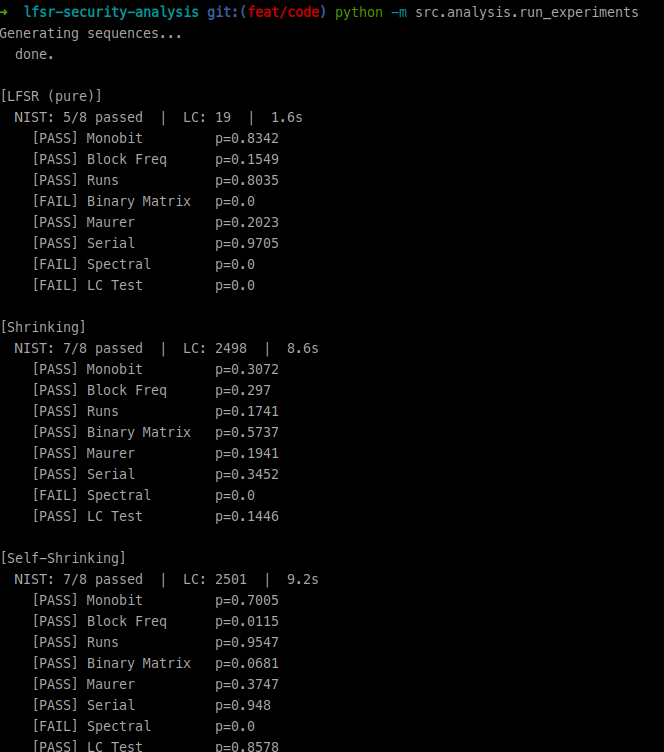
\includegraphics[width=0.9\textwidth]{images/execution_run_experiments_1.png}
\caption{Salida de \texttt{python -m src.analysis.run\_experiments} (parte 1).}
\label{fig:exec-run-experiments-1}
\end{figure}

\begin{figure}[H]
\centering
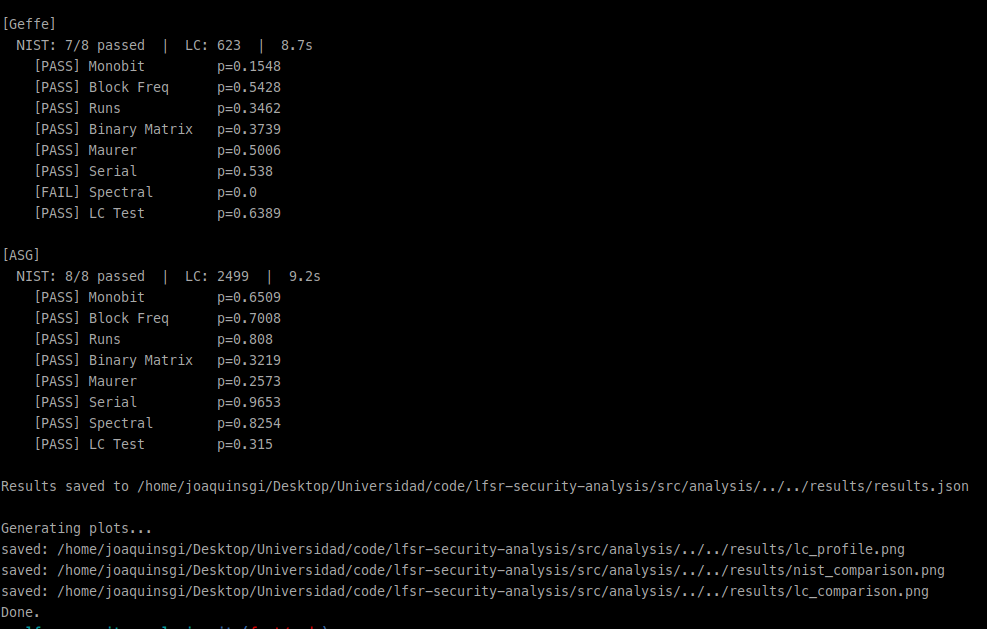
\includegraphics[width=0.9\textwidth]{images/execution_run_experiments_2.png}
\caption{Salida de \texttt{python -m src.analysis.run\_experiments} (parte 2).}
\label{fig:exec-run-experiments-2}
\end{figure}

Cada secuencia tarda unos 10-13 segundos en procesarse. El LFSR puro es el más rápido (1,8 s) porque cae directamente en tres tests sin necesidad de cálculos intensivos.

\subsection{Tabla consolidada}

La tabla~\ref{tab:nist} presenta los p-valores en formato compacto. Los valores en negrita son los que no pasan el umbral $\alpha = 0{,}01$.

\begin{table}[ht]
\centering
\begin{tabular}{l|ccccc}
\hline
\textbf{Test} & \textbf{LFSR} & \textbf{Shrinking} & \textbf{Self-Shr.} & \textbf{Geffe} & \textbf{ASG} \\
\hline
Monobit            & 0,834          & 0,307          & 0,701          & 0,155          & 0,651 \\
Block Freq.        & 0,155          & 0,297          & 0,012          & 0,543          & 0,701 \\
Runs               & 0,804          & 0,174          & 0,955          & 0,346          & 0,808 \\
Binary Matrix      & \textbf{0,000} & 0,574          & 0,068          & 0,374          & 0,322 \\
Maurer             & 0,202          & 0,194          & 0,375          & 0,501          & 0,257 \\
Serial             & 0,971          & 0,345          & 0,948          & 0,538          & 0,965 \\
Espectral          & \textbf{0,000} & \textbf{0,000} & \textbf{0,000} & \textbf{0,000} & 0,825 \\
Complejidad lineal & \textbf{0,000} & 0,145          & 0,858          & 0,639          & 0,315 \\
\hline
\textbf{Pasados}   & 5/8            & 7/8            & 7/8            & 7/8            & 8/8 \\
\textbf{LC medida} & 19             & 2498           & 2501           & 623            & 2499 \\
\hline
\end{tabular}
\caption{P-valores de los ocho tests NIST y complejidad lineal sobre 5.000 bits. Los valores en negrita ($< 0{,}01$) indican tests fallidos.}
\label{tab:nist}
\end{table}

\subsection{Gráficas}

La figura~\ref{fig:lc-bar} compara la complejidad lineal alcanzada por cada generador.
El LFSR puro y el generador de Geffe quedan claramente por debajo de los otros tres,
que se acercan al valor ideal de $N/2 = 2500$ para una secuencia aleatoria de 5.000 bits.

\begin{figure}[H]
\centering
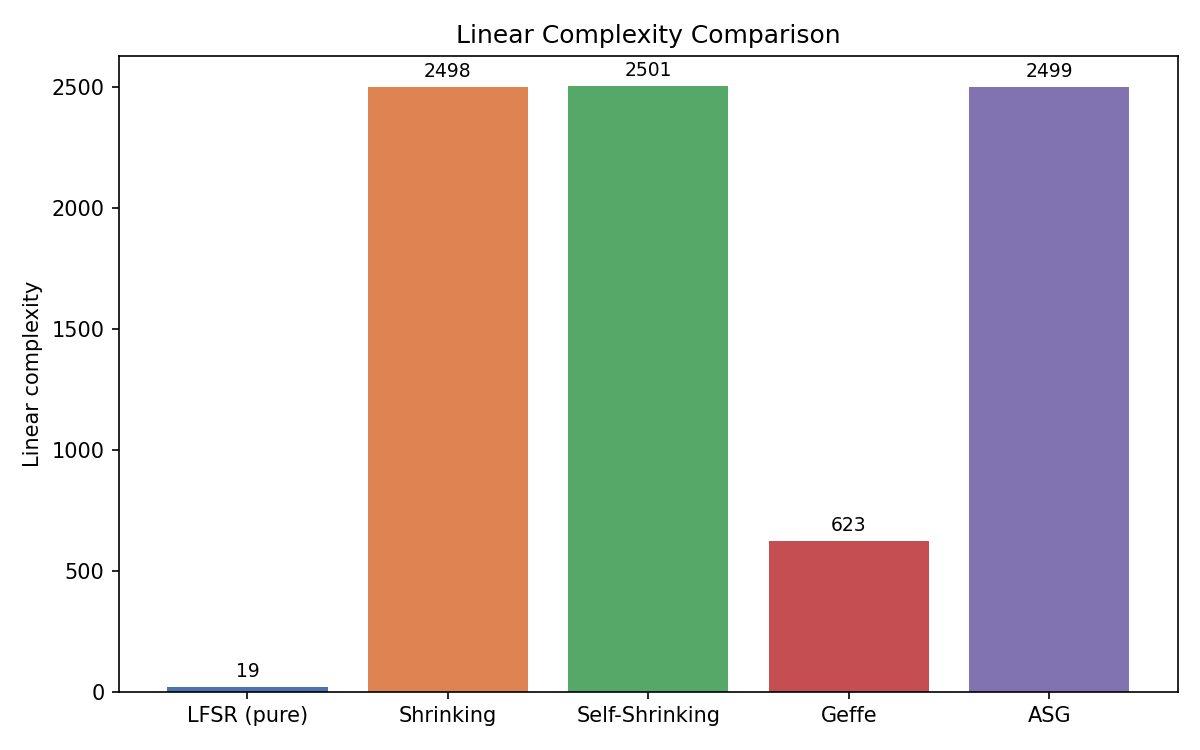
\includegraphics[width=0.8\textwidth]{images/lc_comparison.png}
\caption{Complejidad lineal de cada generador sobre secuencias de 5.000 bits.}
\label{fig:lc-bar}
\end{figure}

El perfil de complejidad lineal (figura~\ref{fig:lc-profile}) muestra cómo evoluciona la complejidad a medida que se procesan más bits.
El LFSR puro se estanca muy pronto en su grado (19), el generador de Geffe crece más despacio que el resto,
y Shrinking, Self-Shrinking y ASG siguen prácticamente la recta $N/2$ esperada de una secuencia aleatoria.

\begin{figure}[H]
\centering
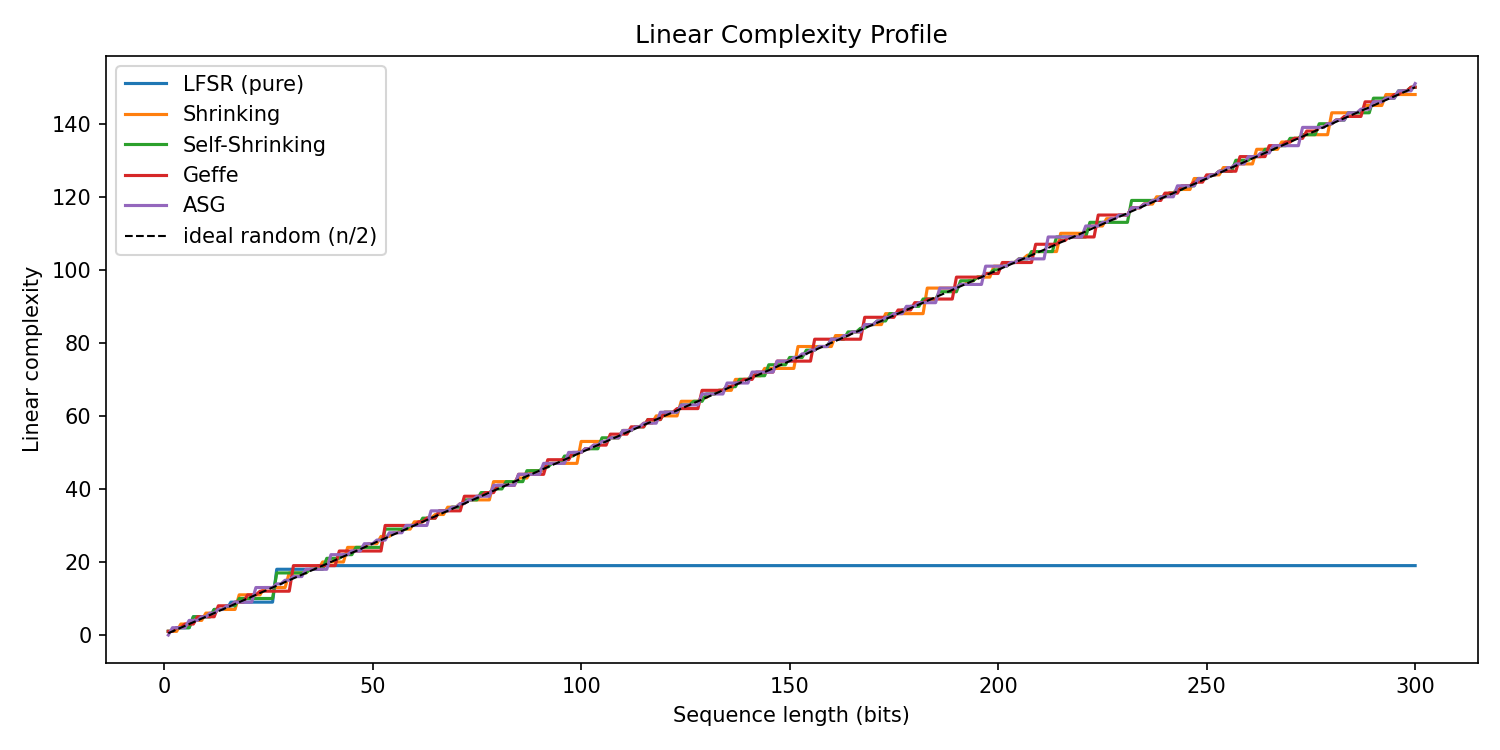
\includegraphics[width=0.85\textwidth]{images/lc_profile.png}
\caption{Perfil de complejidad lineal para los primeros 300 bits de cada generador.
La recta $N/2$ marca el comportamiento esperado de una secuencia aleatoria.}
\label{fig:lc-profile}
\end{figure}

La figura~\ref{fig:nist-comparison} muestra los p-valores de los ocho tests en formato visual.
El generador de ASG (verde) es el único cuyos p-valores se mantienen por encima del umbral en todos los tests. El resto cae en al menos uno.

\begin{figure}[H]
\centering
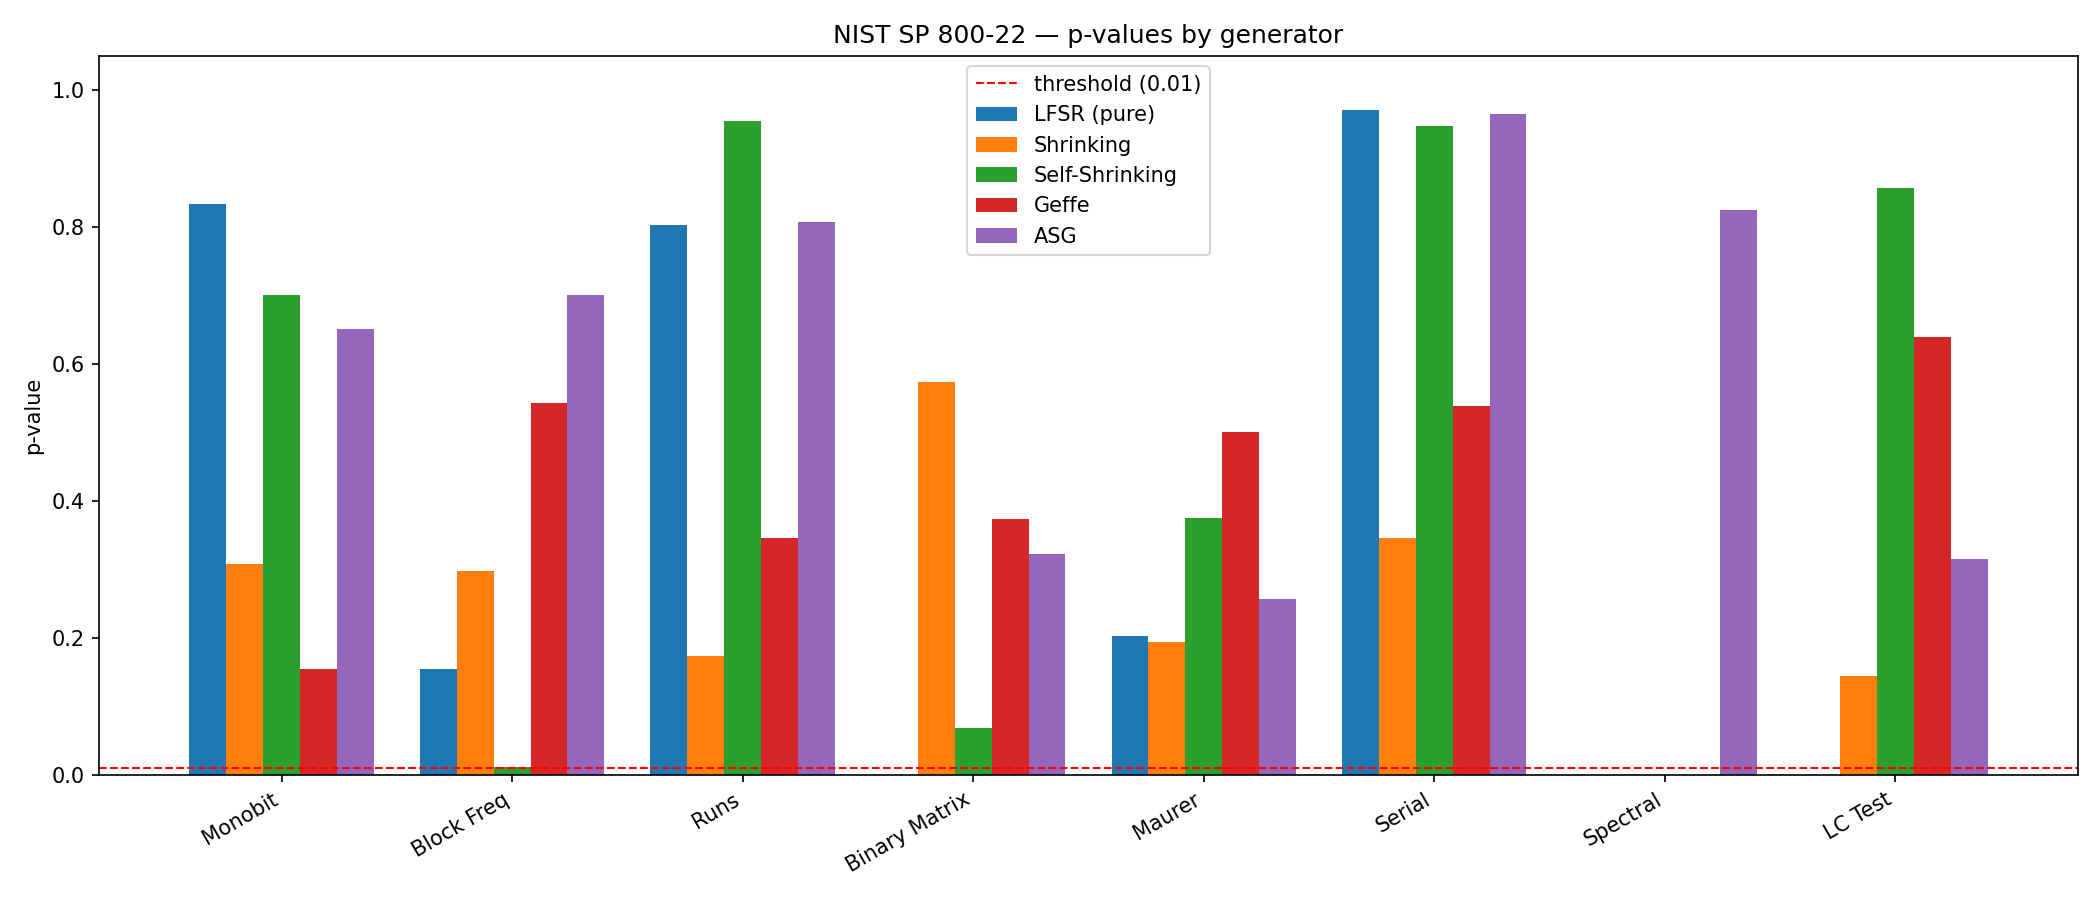
\includegraphics[width=0.95\textwidth]{images/nist_comparison.png}
\caption{P-valores por test y por generador. La línea punteada marca el umbral $\alpha = 0{,}01$.}
\label{fig:nist-comparison}
\end{figure}

\section{Comportamiento con distintos tamaños de secuencia}
\label{sec:multi-size}

Los resultados anteriores corresponden a una longitud de secuencia concreta.
Para ver cómo dependen del tamaño, repito los experimentos con $n \in \{1000, 5000, 10000, 50000\}$
midiendo la complejidad lineal y los p-valores de tres tests representativos,
Monobit (balance global), Runs (estructura local) y Espectral (periodicidad).

El script \texttt{multi\_size.py} hace exactamente eso, genera las cinco secuencias para cada $n$ y va imprimiendo los resultados en formato tabla.

\begin{figure}[H]
\centering
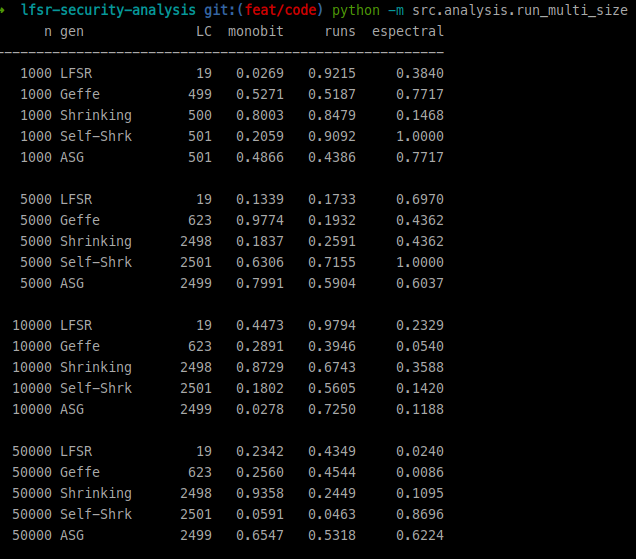
\includegraphics[width=0.9\textwidth]{images/execution_multi_size.png}
\caption{Salida de \texttt{python -m src.analysis.run\_multi\_size}.}
\label{fig:exec-multi-size}
\end{figure}

Hay tres patrones interesantes que se ven de un vistazo en estos datos.

Primero, la \textbf{complejidad lineal del LFSR puro se queda anclada en 19} por mucho que se alargue la secuencia.
Es exactamente lo que predice la teoría, da igual ver 1000 o 50000 bits, Berlekamp-Massey siempre devuelve el grado del registro.
Esa estabilidad es la firma de una secuencia lineal.

Segundo, los generadores no triviales saturan la complejidad lineal en valores cercanos a $N/2$.
Con $n = 1000$ todos rondan 500, con $n = 5000$ rondan 2500 (excepto Geffe, que se queda en 623).
La cota $\Lambda \leq \lfloor N/2 \rfloor$ se cumple siempre y se saturan a partir de cierta longitud porque la complejidad lineal se calcula sobre los primeros 5000 bits.

Tercero, el \textbf{test espectral se vuelve más estricto cuando la secuencia crece}.
Con $n = 1000$ casi cualquier generador lo pasa cómodamente. Con $n = 50000$, el LFSR puro y Geffe
empiezan a quedar peligrosamente cerca del umbral (0,024 y 0,0086 respectivamente),
y a partir de aquí esperaríamos que cayeran por debajo. Esto es coherente con lo que vimos antes en la tabla principal,
con secuencias de 500.000 bits los cuatro generadores excepto el ASG fallan el espectral con p-valor 0.

\section{Validación del software}
\label{sec:validacion}

Antes de fiarse de los p-valores reportados conviene verificar que el código no contiene errores.
Cada componente del repositorio tiene su batería de tests unitarios con \texttt{pytest},
que comprueba contra valores conocidos. Los tests cubren tres áreas.

\begin{itemize}
  \item \textbf{LFSR} (7 tests). Periodo máximo con polinomios primitivos de grado 5 y 7,
        salida binaria, reset del estado, validación de errores en el constructor
        (estado todo-ceros, longitud incorrecta, bits inválidos).
  \item \textbf{Berlekamp-Massey} (6 tests). Complejidad lineal de una m-sequence igual al grado del LFSR original,
        reconstrucción del LFSR a partir de $2n$ bits, secuencia constante con $\Lambda = 1$,
        secuencia alternante con $\Lambda = 2$, perfil de complejidad no decreciente,
        polinomio recuperado con $c_0 = 1$.
  \item \textbf{Generadores} (14 tests). Longitud de salida correcta, salida binaria,
        complejidad lineal mayor que la de los componentes y determinismo
        (la misma semilla produce la misma secuencia) para cada uno de los cuatro generadores.
\end{itemize}

Al ejecutar \texttt{pytest} sobre el árbol completo, los 27 tests pasan en menos de un segundo.

\begin{figure}[H]
\centering
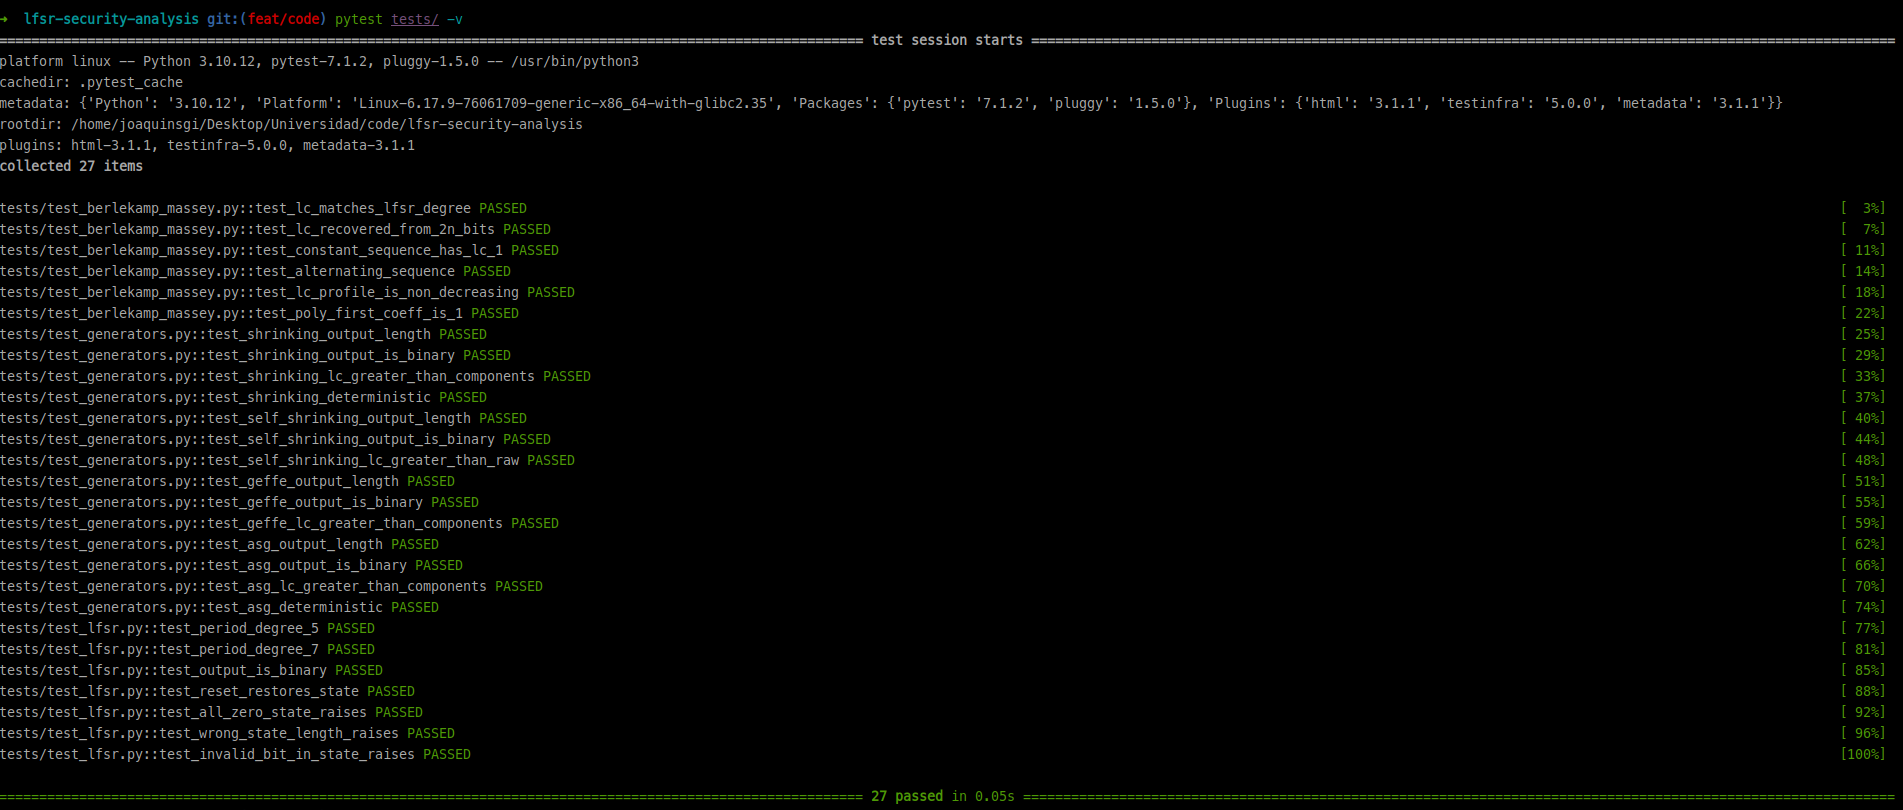
\includegraphics[width=0.9\textwidth]{images/execution_pytest.png}
\caption{Salida de \texttt{pytest tests/ -v}.}
\label{fig:exec-pytest}
\end{figure}

Esto no demuestra que la implementación sea correcta en sentido formal, ya que los tests cubren casos conocidos y no exhaustividad.
Pero sí da confianza razonable en que los p-valores de la tabla principal no son artefactos de un bug, sobre todo cuando los valores observados
coinciden cualitativamente con lo que predice la teoría (LFSR puro con LC igual al grado, Geffe con LC moderada, etc.).

Cuando uno de los resultados experimentales sorprendía (por ejemplo el p-valor de 0,012 del Self-Shrinking
en Block Frequency, ajustadísimo al umbral), poder ir al código del test y revisar paso a paso qué hacía el cálculo era exactamente lo que justifica
haber implementado todo desde cero en vez de tirar de librerías.

\section{Análisis por generador}

\subsection{LFSR puro}

Pasa 5 de 8 tests. Los tres que falla (Binary Matrix, Espectral y Complejidad lineal)
son precisamente los tres que detectan estructura lineal. Los cinco que pasa (Monobit, Block Frequency, Runs, Maurer y Serial)
evalúan propiedades estadísticas que las m-sequences cumplen de forma natural por las propiedades de Golomb.

Esto es importante, ya que si solo se mira con tests estadísticos básicos un LFSR puro \textit{parece} aceptable.
La diferencia entre apariencia y realidad se ve en su perfil de complejidad lineal, plano desde el bit 38 en adelante.
Y eso es exactamente lo que Berlekamp-Massey explota.

\subsection{Geffe}

Pasa 7 de 8 tests, con el espectral como único fallo. Estadísticamente se comporta bastante bien.
Pero recordemos del capítulo anterior, el problema real del generador de Geffe es la correlación $0{,}75$ con dos de los tres LFSR,
no la estadística de su salida. Un atacante no necesita aplicar Berlekamp-Massey,
puede romper cada registro por separado con coste $2^7 + 2^5 + 2^9 = 672$ operaciones para nuestros tamaños.

Lo curioso es que los tests NIST no detectan esa vulnerabilidad. Esto es importante, los tests evalúan calidad estadística,
no resistencia a ataques estructurales.

\subsection{Shrinking y Self-Shrinking}

Ambos generadores pasan 7 de 8 tests, fallando solo el espectral. Sus complejidades lineales son excelentes (2498 y 2501, prácticamente $N/2$).
Desde el punto de vista de Berlekamp-Massey son tan buenos como una secuencia aleatoria.

El fallo del espectral tiene una explicación intuitiva, la secuencia base sigue siendo la de un LFSR,
y aunque el muestreo irregular dispersa los picos espectrales del registro original,
no los elimina del todo. La DFT todavía detecta exceso de picos por encima del umbral teórico.

Es una debilidad teórica que no compromete la seguridad práctica (no se conocen ataques que exploten esta periodicidad residual),
pero es un detalle medible. En la práctica esto desaparece con LFSR de grado mayor, ya que los armónicos se diluyen en secuencias largas.

El Self-Shrinking además tiene el p-valor de block frequency más justo (0,012), muy cerca del umbral.
Esto sugiere que la selección irregular sobre la propia secuencia introduce algún desequilibrio local,
posiblemente porque selector y datos no son independientes.

\subsection{ASG}

Único que pasa los 8 tests con los parámetros usados. Su p-valor en el test espectral (0,825) no solo está por encima del umbral
sino que es alto incluso para una secuencia aleatoria. Eso indica que el mecanismo del ASG hace un trabajo particularmente bueno destruyendo periodicidades.

Lo más interesante es que el de ASG usa los mismos tres LFSR que el de Geffe. Mismo hardware, complejidad lineal 4x mayor y todos los tests pasados.
Reloj alterno con XOR de fuentes independientes funciona mucho mejor que un multiplexor de selección directa.

\section{Discusión}

\subsection{La complejidad lineal es necesaria pero no suficiente}

La tabla de resultados separa muy claramente a los generadores en dos grupos. En el primero, LFSR puro y Geffe,
con complejidad lineal baja (19 y 623). En el segundo, Shrinking, Self-Shrinking y ASG, con complejidad lineal cercana a $N/2$.

Sin embargo, dentro del segundo grupo la complejidad lineal sola no permite distinguir nada.
Los tres tienen valores prácticamente idénticos ($\sim 2500$) pero comportamiento muy distinto en el test espectral.
Tener complejidad lineal alta es condición necesaria (un generador con LC baja cae frente a Berlekamp-Massey) pero no garantiza calidad estadística completa.

\subsection{Los tests estadísticos no detectan todo}

El caso de Geffe es ilustrativo, pasa 7 de 8 tests pese a ser trivialmente atacable por correlación.
Los tests NIST detectan desviaciones estadísticas de la salida, pero no analizan la estructura interna del generador.
Para evaluar un generador hace falta combinar tests estadísticos, complejidad lineal y análisis de ataques específicos.

\subsection{El mecanismo de combinación es lo que importa}

La comparación Geffe vs ASG es la más reveladora del trabajo. Mismos LFSR, mismos polinomios, mismos estados iniciales.
La única diferencia es cómo se combinan, multiplexor vs reloj alterno con XOR.
El resultado, Geffe falla espectralmente y tiene correlación 0,75, ASG pasa todos los tests y no tiene correlación detectable.

Esta es probablemente la lección de diseño más clara del experimento.
En generadores basados en LFSR la clave no es el tamaño de los registros sino el mecanismo de combinación.

\section{Limitaciones del análisis}

Conviene tener presente lo que este análisis no cubre.

\textbf{Un solo estado inicial por generador.} Los resultados corresponden a una ejecución
con estados fijos. Para los p-valores cerca del umbral (como el 0,012 del Self-Shrinking en block frequency)
otro estado inicial podría dar resultados distintos. Un análisis más robusto repetiría con varios estados
y reportaría la distribución de p-valores.

\textbf{Tests no implementados.} Faltan 7 de los 15 tests del estándar.
Random excursions en particular podría detectar asimetrías que los implementados no cubren.

\textbf{Ataques no implementados.} El ataque de correlación contra Geffe se describe en teoría
pero no se ejecuta. Una extensión natural sería programarlo y verificar
que el coste real coincide con el predicho.

Pese a estas limitaciones, los resultados son coherentes con la teoría y permiten extraer conclusiones claras sobre la seguridad relativa de los cuatro generadores,
que es lo que se discute en el capítulo final.
